\documentclass[12pt]{article}

\usepackage{sbc-template}
\usepackage{graphicx,url}
\usepackage[utf8]{inputenc}
\usepackage[brazil]{babel}
\usepackage{pgfplots}
\pgfplotsset{compat=1.18}

     
\sloppy

\title{Mapa Cidadão: Uma Aplicação De Crowdsourcing Com Ênfase Em Espaciabilidade}

\author{
Mateus Vinicius S. Melo\inst{1},
André Avelino da Silva Neto\inst{1},
Marcelle Pereira Mota\inst{1}
}


\address{Instituto de Ciências Exatas e Naturais -- Faculdade de Computação -- \\
    Universidade Federal do Pará (UFPA)\\
  CEP 66075-110 -- Belém/PA –– Brasil
\email{ \{mateus.melo,andre.neto\}@icen.ufpa.br, mpmota@ufpa.br }
}

\begin{document}

\maketitle

\begin{abstract}
  This article presents Mapa Cidadão, a collaborative urban mapping system developed from the concept of spatiality, understood as the ability of cartographic interfaces to support spatial reasoning. In addition to the system's construction, an evaluation was conducted using a spatiality assessment method with experts in Human-Computer Interaction (HCI) and design, the MIE. The evaluation aimed to assess both the application and the method itself, as well as its production of specific results. Spatability was identified as a relevant evaluation criterion for collaborative mapping systems, but one that still maintains a strong interdependence with other HCI quality criteria, such as usability and user experience.
\end{abstract}
     
\begin{resumo} 
Este artigo apresenta o Mapa Cidadão, um sistema colaborativo de mapeamento urbano desenvolvido a partir do conceito de espaciabilidade, entendido como a capacidade de interfaces cartográficas apoiarem o raciocínio espacial. Além da construção do sistema, foi conduzida uma avaliação utilizando um método de avaliação da espaciabilidade com especialistas da área de Interação Humano-Computador (IHC) e design, o MIE. Durante a avaliação buscou-se tanto avaliar a aplicação quanto o próprio método e sua produção de resultados específicos. Identificou-se a espaciabilidade como um critério relevante de avaliação para sistemas de mapas colaborativos, mas que ainda mantêm uma forte interdependência entre outros critérios de qualidade em IHC, como usabilidade e experiência do usuário.
\end{resumo}


\section{Introdução}

Tecnologias digitais baseadas em georreferenciamento têm se tornado centrais no contexto urbano, especialmente para o registro e o compartilhamento de informações sobre problemas relacionados à infraestrutura, serviços públicos e condições ambientais. A popularização de dispositivos móveis conectados à Internet e de plataformas participativas tem ampliado a produção colaborativa de dados espaciais, fortalecendo iniciativas de participação cidadã mediadas por sistemas de informação \cite{estelles:2015,alter:2018}.

Nesse cenário, práticas de \textit{crowdsourcing} são amplamente adotadas em aplicações de mapeamento colaborativo urbano, sendo reconhecidas por seu potencial de apoio à governança urbana, à transparência pública e às tecnologias cívicas \cite{gonzaga:2025,torquato:2024}. Entretanto, grande parte dessas aplicações ainda se concentra no registro e na visualização pontual de ocorrências, utilizando o mapa principalmente como recurso de localização. Esse enfoque limita a interpretação dos dados espaciais, dificultando a identificação de padrões, áreas críticas e associações entre diferentes problemas urbanos.

O problema abordado neste trabalho refere-se à lacuna entre a coleta colaborativa de dados georreferenciados e o apoio efetivo ao raciocínio espacial dos usuários. Estudos indicam que a simples disponibilização de dados em mapas não garante compreensão territorial, sendo necessário considerar como decisões de design, interação e representação cartográfica influenciam a interpretação espacial \cite{haklay:2012,see:2016}.

Diante desse contexto, este trabalho adota o conceito de espaciabilidade como referencial teórico para orientar o desenvolvimento e a avaliação de aplicações cartográficas interativas. A espaciabilidade é entendida como a capacidade da interface de apoiar a compreensão e a interpretação dos dados espaciais, auxiliando o usuário na geração de insights e na tomada de decisão \cite{neto:ihc}.

Este artigo apresenta o desenvolvimento e a avaliação inicial do \textit{Mapa Cidadão}, configurando-se como uma pesquisa em andamento. O objetivo da pesquisa é demonstrar como o conceito de espaciabilidade pode orientar a concepção de uma aplicação de \textit{crowdsourcing} urbano desde sua origem, bem como aplicar empiricamente o Método de Inspeção da Espaciabilidade (MIE) em um estudo preliminar com três participantes. Como contribuições parciais, o trabalho operacionaliza um conceito teórico no desenvolvimento de um sistema real e apresenta evidências iniciais sobre sua aplicação, discutindo limitações e apontando direções para investigações futuras.





\section{Fundamentação Teórica}

Esta seção apresenta os conceitos que fundamentam o desenvolvimento e a avaliação do Mapa Cidadão, abrangendo \textit{crowdsourcing}, georreferenciamento, participação cidadã digital e o conceito de espaciabilidade em interfaces baseadas em mapas.

\subsection{Crowdsourcing e Georreferenciamento}

O \textit{crowdsourcing} caracteriza-se como uma abordagem na qual atividades tradicionalmente atribuídas a especialistas passam a ser realizadas de forma distribuída por um grande número de indivíduos, geralmente mediadas por plataformas digitais. 

No contexto urbano, o uso de \textit{crowdsourcing} associado ao georreferenciamento possibilita a coleta colaborativa de informações relacionadas à infraestrutura, mobilidade e serviços públicos, ampliando significativamente a cobertura espacial e a frequência de atualização dos dados disponíveis \cite{sui:2013,haklay:2012}. 


Essas práticas impulsionam o desenvolvimento de plataformas de participação cidadã digital e tecnologias cívicas, nas quais cidadãos contribuem ativamente para a construção coletiva de informações sobre a cidade. Tais iniciativas buscam fortalecer o engajamento social, ampliar a transparência e apoiar processos de compreensão urbana baseados em dados produzidos pela própria população \cite{gonzaga:2025,afzalan:2017}. No entanto, a efetividade dessas plataformas não depende apenas da coleta de dados, mas também da forma como as informações são organizadas, representadas e disponibilizadas para interpretação pelos usuários.




\subsection{Qualidade em Interação Humano-Computador e Espaciabilidade}
A Interação Humano-Computador (IHC), em geral, enfatiza estudos que priorizam o papel do usuário na interação com sistemas. Critérios de qualidade em IHC apoiam atividades de avaliação de interfaces sob diferentes perspectivas \cite{barbosa2010interaccao}. A usabilidade, por exemplo, relaciona-se à eficácia e eficiência na realização de tarefas, enquanto a Experiência do Usuário (UX) incorpora dimensões subjetivas, como percepção, engajamento e significado da interação.

Embora esses critérios sejam fundamentais, eles não abordam explicitamente o suporte ao raciocínio espacial em interfaces baseadas em mapas. Nesse contexto, surge o conceito de espaciabilidade, entendido como a capacidade de uma interface cartográfica apoiar processos de compreensão e interpretação de dados espaciais \cite{neto:ihc}. A espaciabilidade pode ser caracterizada como um novo critério de qualidade em IHC, oferecendo uma perspectiva relacionada a interpretação e apoio a tomadas de decisão com base nos dados espaciais.



Para operacionalizar esse conceito, Neto e Mota \cite{neto:ihc} propõem o Método de Inspeção da Espaciabilidade (MIE), baseado na análise por especialistas em IHC ou design. No método, os especialistas conduzem tarefas no sistema alvo da avaliação, simulando o papel de um usuário final. O método organiza a avaliação em dimensões analíticas que orientam a formulação das tarefas e a identificação de barreiras ao raciocínio espacial. As dimensões incluem: (D1) orientação e direção; (D2) padrões espaciais; (D3) decisão sobre localização ideal; (D4) associações espaciais; (D5) sobreposição de camadas; e (D6) interpretação de tipos espaciais.



O MIE é estruturado em etapas sequenciais que orientam sua aplicação prática. Inicialmente, realiza-se a definição dos objetivos da aplicação avaliada (1), identificando quais dimensões de espaciabilidade são mais relevantes ao contexto de uso. Em seguida, são definidos cenários de avaliação (2), que pode incluir a elaboração de personas e a proposição de uma ou mais tarefas associadas a cada dimensão selecionada. Posteriormente, os especialistas conduzem a execução simulada das tarefas (3) na interface, observando possíveis barreiras ao raciocínio espacial. A quarta etapa consiste na produção de relatórios de inspeção (4), nos quais são registrados os problemas identificados, suas descrições e possíveis recomendações. Por fim, procede-se à análise dos resultados (5), buscando interpretar de forma integrada como o design da aplicação apoia — ou limita — a espaciabilidade. Ressalta-se que o MIE é proposto como um rascunho teórico inicial, no qual os autores incentivam que seja validado e aprimorado por pesquisas empíricas \cite{neto:ihc}, o que é feito na presente pesquisa.





\section{Trabalhos Relacionados}

Diversos trabalhos investigam o uso de mapas colaborativos e dados georreferenciados produzidos por cidadãos para a representação de fenômenos urbanos. A literatura sobre \textit{Volunteered Geographic Information} (VGI) destaca o papel do usuário como produtor voluntário de dados espaciais, ampliando a cobertura e a atualização das informações geográficas \cite{sui:2013}. Iniciativas consolidadas, como o OpenStreetMap, exemplificam esse paradigma ao fornecer uma base cartográfica colaborativa amplamente utilizada \cite{haklay:2012}.

No contexto do registro de problemas urbanos e situações de crise, plataformas como o Ushahidi demonstram o potencial do \textit{crowdsourcing} georreferenciado para engajar cidadãos e visualizar eventos no território \cite{meier:2015}. Contudo, grande parte dessas soluções utiliza o mapa principalmente como suporte visual ao registro das ocorrências, oferecendo apoio limitado à análise espacial mais aprofundada. Estudos sobre tecnologia cívica ressaltam o impacto dessas plataformas no engajamento social, mas também apontam desafios relacionados à validação dos dados e à limitada exploração de padrões e associações espaciais \cite{gonzaga:2025}.

Pesquisas em IHC e geovisualização têm enfatizado a importância da cognição na interpretação de mapas e dados espaciais. Trabalhos clássicos destacam que processos como percepção, atenção e raciocínio espacial influenciam diretamente a usabilidade de sistemas cartográficos \cite{slocum2001cognitive,montello2009cognitive}. Esses estudos indicam a necessidade de abordagens metodológicas que conectem usabilidade e cognição espacial de forma mais explícita, especialmente em aplicações interativas baseadas em mapas.

Nesse contexto, o conceito de espaciabilidade surge como uma abordagem para analisar como o design de interfaces cartográficas apoia operações de orientação, identificação de padrões e associações espaciais \cite{neto:ihc}. Entretanto, ainda são escassos os sistemas de mapeamento colaborativo urbano que incorporam esse conceito de forma sistemática, tanto no projeto quanto na avaliação. Diferenciando-se dos trabalhos relacionados, o Mapa Cidadão integra \textit{crowdsourcing}, georreferenciamento e espaciabilidade ao tratar o mapa como um artefato cognitivo voltado à interpretação espacial das ocorrências urbanas, sendo avaliado por meio de dimensões analíticas específicas (D1–D6), o que contribui para preencher uma lacuna identificada na literatura.


\section{Procedimentos Metodológicos}
Os procedimentos metodológicos adotados neste estudo foram definidos visando 
avaliar o Mapa Cidadão enquanto uma aplicação colaborativa de mapeamento urbano, com ênfase na espaciabilidade. A abordagem metodológica possui caráter qualitativo e exploratório, investigando percepções, interpretações e estratégias cognitivas mobilizadas pelos usuários durante a interação com interfaces baseadas em mapas, conforme recomendado em estudos da área de IHC \cite{silveira:2024}. A metodologia foi estruturada em um conjunto de etapas sequenciais e interdependentes, que contemplam desde o desenvolvimento do sistema até a análise dos dados empíricos obtidos durante a avaliação. Essas etapas estão sintetizadas na Figura~\ref{fig:figura-etapas}, que apresenta uma visão geral do fluxo metodológico adotado no estudo.

\begin{figure}[ht]
    \centering
    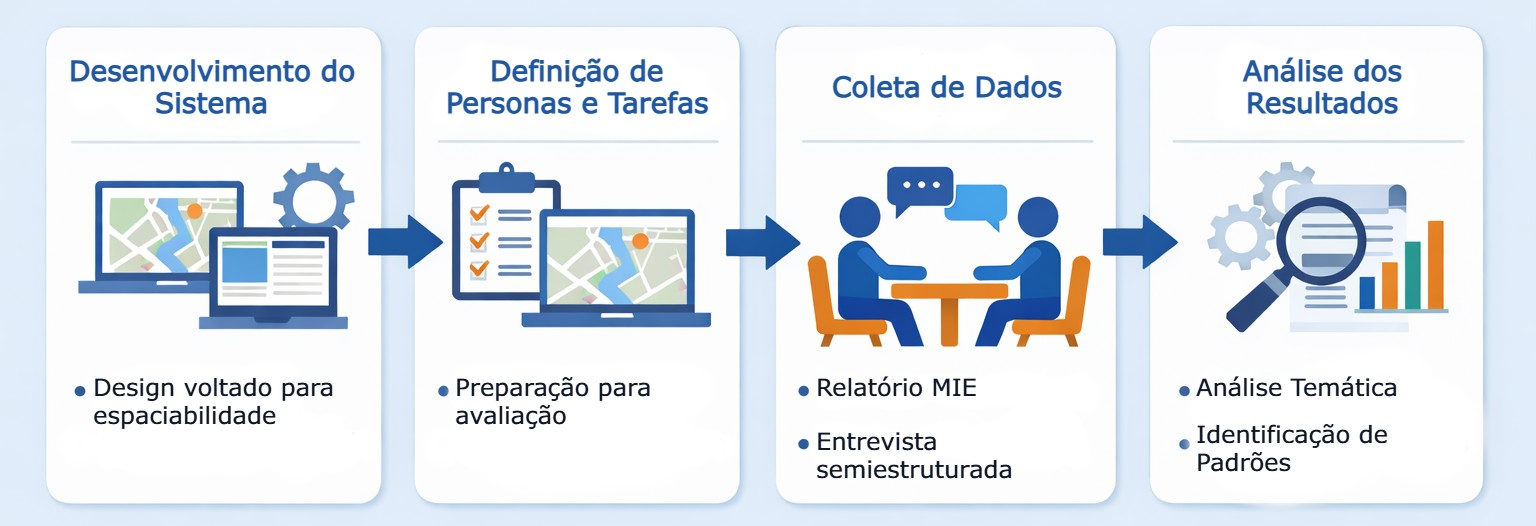
\includegraphics[width=0.6\linewidth]{figuras/figura_etapas_3.jpg}
    \caption{Etapas da metodologia adotada no estudo.}
    \label{fig:figura-etapas}
\end{figure}

\subsection{Desenvolvimento do Sistema}

O Mapa Cidadão é um sistema colaborativo de registro e visualização de ocorrências urbanas, baseado em \textit{crowdsourcing} e georreferenciamento, tendo a espaciabilidade como diretriz central de projeto. Desde sua concepção, buscou-se estruturar a interface não apenas como um repositório de registros, mas como um ambiente capaz de favorecer orientação espacial, identificação de padrões e interpretação de relações territoriais.

\begin{figure}[ht]
    \centering
    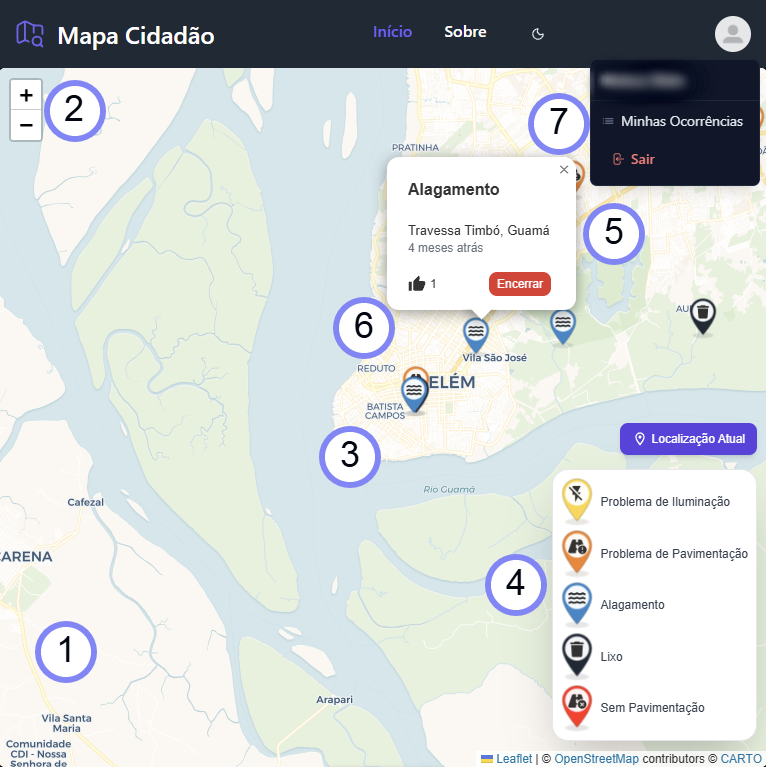
\includegraphics[width=0.6\linewidth]{figuras/figura_mapa_cidadao_2.png}
    \caption{Tela inicial do projeto.}
    \label{fig:figura-1}
\end{figure}

A Figura~\ref{fig:figura-1} ilustra a tela inicial do Mapa Cidadão. A interface é organizada em torno de um mapa interativo que ocupa a região central da tela (1), permitindo navegação por meio de zoom e deslocamento (2). As ocorrências são representadas por marcadores geográficos diferenciados por ícones e cores, associados a categorias como alagamento, iluminação pública, lixo e pavimentação (3). Uma legenda integrada auxilia na interpretação dos símbolos (4), apoiando a distinção entre tipos de problema — elemento diretamente relacionado à dimensão D6 de espaciabilidade (interpretação de tipos espaciais). Ao clicar em um marcador, o usuário acessa informações detalhadas sobre a ocorrência, incluindo tipo do problema , endereço aproximado e estado do registro, articulando localização geográfica e conteúdo informacional (5).

O sistema também incorpora funcionalidades colaborativas, como a possibilidade de registrar novas ocorrências, interagir com registros existentes por meio de um mecanismo de validação (“like”) e encerrar ocorrências (6). O acesso às funcionalidades depende de autenticação, sendo necessário realizar login para cadastrar registros. Há ainda um menu de perfil que reúne informações do usuário e o histórico de “Minhas ocorrências”, permitindo o acompanhamento das contribuições individuais (7). Essas decisões de design buscaram alinhar-se às dimensões do MIE consideradas mais relevantes diante do objetivo do Mapa Cidadão, em especial as dimensões D1, D2, D4 e D6. No entanto, o sistema, em sua versão avaliada, não incorporava mecanismos avançados de filtragem, agregação ou visualização analítica, operando principalmente com a visualização simultânea de marcadores distribuídos no território. Essa configuração foi relevante para a análise posterior por influenciar diretamente as percepções dos especialistas quanto ao suporte ao raciocínio espacial.





\subsection{Definição de Personas e Tarefas}


A segunda etapa da pesquisa consistiu na definição de personas e tarefas para a avaliação e validação do Mapa Cidadão. O processo de avaliação proposto considerou principalmente a espaciabilidade como critério de qualidade, devido ao objetivo geral de estimular a compreensão dos dados espaciais e a produção de ideias sobre os dados. Por conta disso, o MIE \cite{neto:ihc} foi utilizado nesta etapa como base para o planejamento desta avaliação. Dessa forma, as definições dessa etapa seguem a proposta do método.

Inicialmente, foram identificadas, a partir dos objetivos de uso da aplicação, quais dimensões de espaciabilidade deveriam ser priorizadas para avaliação. A dimensão D1 (compreensão de orientação e direção) foi selecionada por possibilitar a avaliação do suporte oferecido pelo sistema à localização das ocorrências e à orientação do usuário no território. A dimensão D2 (detecção de padrões espaciais) foi incluída por permitir analisar se a organização visual das ocorrências favorece identificar concentrações e recorrências de problemas urbanos. A dimensão D4 (identificação de associações espaciais) foi adotada para analisar a capacidade do usuário de relacionar diferentes tipos de ocorrências. Por fim, a dimensão D6 (interpretação de tipos espaciais) foi selecionada para avaliar se a simbologia empregada — ícones, cores e marcadores — permite distinguir adequadamente os diferentes tipos de ocorrências representadas no mapa.

Para contextualizar as tarefas em situações próximas ao uso real, foram definidas duas personas representativas de perfis potenciais de usuários do sistema: \textbf{João}, 40 anos, morador de um bairro periférico. Ele utiliza o Mapa Cidadão para registrar ocorrências próximas à sua residência, como iluminação pública defeituosa e buracos na via. Seu principal interesse é acompanhar se os problemas reportados são recorrentes e se há providências por parte do poder público. E \textbf{Ana}, 27 anos, estudante universitária, ela utiliza o sistema para consultar ocorrências já registradas na região onde mora e, eventualmente, criar novos registros, como acúmulo de lixo ou alagamentos. Seu objetivo é compreender como esses problemas afetam sua mobilidade e qualidade de vida no bairro.

%\subsubsection{Tarefas de avaliação}

Com as personas e os objetivos definidos, foram elaboradas tarefas específicas em cenários para avaliar diferentes dimensões de espaciabilidade. Os cenários foram: (i) João deseja localizar todas as ocorrências de iluminação no bairro dele (D1); (ii) Ana quer identificar quais áreas da cidade apresentam maior número de alagamentos (D2); (iii) João tenta perceber se os problemas de falta de pavimentação registrados no seu bairro estão relacionados a ocorrências de alagamentos (D4); e (iv) Ana precisa compreender claramente cada marcador no mapa (D6).

\subsection{Coleta de Dados}

Dando prosseguimento à condução do Método de Inspeção da Espaciabilidade (MIE), foi realizada a etapa de coleta dos dados avaliativos. Para essa fase, foram convidados três especialistas na área de Interação Humano-Computador (IHC), identificados como P1, P2 e P3, responsáveis por executar as tarefas definidas no sistema Mapa Cidadão, incorporando as personas propostas para orientar suas decisões ao longo da avaliação. A escolha por três participantes fundamenta-se na condução de uma análise qualitativa aprofundada da aplicação, permitindo a comparação entre os resultados obtidos e a verificação do potencial do método em produzir achados consistentes e replicáveis entre diferentes avaliadores.

Os participantes da pesquisa eram estudantes de pós-graduação stricto sensu em Ciência da Computação, vinculados a um laboratório de pesquisa em IHC de uma universidade pública. O participante P1 é do sexo feminino, possui três anos de experiência na área de IHC e cursava mestrado em Ciência da Computação. O participante P2 é do sexo masculino, possui seis anos de experiência em IHC e cursava doutorado na área. O participante P3, também do sexo masculino, possui quatro anos de experiência em IHC e cursava doutorado. Embora os participantes integrassem o mesmo grupo de pesquisa e se conhecessem previamente, todos foram explicitamente orientados a realizar a avaliação de forma independente, sem comunicação ou troca de informações durante o processo, com o objetivo de minimizar possíveis influências mútuas nos resultados.

Ressalta-se que nenhum dos participantes possuía familiaridade prévia com o conceito de espaciabilidade ou com o Método de Inspeção da Espaciabilidade (MIE), tampouco havia tido contato anterior com o sistema Mapa Cidadão, o que contribuiu para uma avaliação mais isenta e alinhada ao ponto de vista de especialistas externos ao domínio específico do método e da aplicação.

No que se refere à experiência com aplicações cartográficas, os participantes P1 e P3 relataram não possuir vivência profissional ou acadêmica em design de sistemas baseados em mapas, restringindo sua experiência ao uso cotidiano de aplicações como Google Maps e Waze para fins de mobilidade urbana. O participante P2, por sua vez, informou experiência adicional no design de sistemas de \textit{crowdsourcing} georreferenciado, bem como participação em pesquisas na área de IHC voltadas a aplicações cartográficas, com ênfase em acessibilidade de interfaces.

Após a entrega dos relatórios individuais resultantes da aplicação do MIE, foi conduzida uma entrevista semiestruturada com cada participante, realizada de forma remota e individual. As entrevistas tiveram como objetivo complementar e aprofundar os dados obtidos nos relatórios escritos, possibilitando uma compreensão mais detalhada sobre (i) a percepção dos especialistas em relação ao sistema avaliado (Mapa Cidadão) e (ii) a avaliação do próprio Método de Inspeção da Espaciabilidade enquanto instrumento metodológico. Todas as entrevistas foram gravadas, mediante consentimento prévio dos participantes, para posterior análise qualitativa.

O roteiro das entrevistas foi estruturado em três eixos principais. O primeiro eixo teve como finalidade contextualizar o perfil dos participantes, por meio de questões relacionadas à experiência prévia com mapas interativos e geoinformação, permitindo interpretar suas análises à luz de seus repertórios técnicos e práticos. O segundo eixo concentrou-se na avaliação da aplicação, abordando aspectos como a primeira impressão sobre a proposta do Mapa Cidadão, a percepção do mapa enquanto visualizador de ocorrências ou ferramenta analítica, a identificação de elementos de design que potencializavam ou limitavam a espaciabilidade, bem como sugestões gerais de melhoria. O terceiro eixo voltou-se à avaliação do próprio MIE, investigando a adequação das tarefas propostas, sua relação com situações reais e relevantes para a compreensão espacial e possíveis sugestões de aprimoramento do método. A inclusão desse eixo justifica-se pela necessidade de avaliar não apenas os resultados da aplicação, mas também a validade, a aplicabilidade prática e o potencial de refinamento do método proposto.



\subsection{Análise dos Resultados}

Os dados dos relatórios produzidos pelos participantes e das entrevistas semiestruturadas foram examinados por meio de análise temática, técnica amplamente empregada na investigação qualitativa para identificar, organizar e interpretar padrões de significado em conjuntos de dados textuais \cite{rosa:2021}. Adotou-se uma abordagem dedutiva, na qual as categorias analíticas foram previamente definidas com base nos objetivos da pesquisa. Assim, o material coletado foi organizado em quatro eixos principais: (i) espaciabilidade, (ii) usabilidade, (iii) experiência do usuário (UX) e (iv) avaliação do Método de Inspeção da Espaciabilidade (MIE). Trechos relevantes dos relatórios e excertos das falas dos participantes foram codificados e alocados nas respectivas categorias, permitindo sistematizar as evidências empíricas conforme os critérios investigados.

Essa estratégia possibilitou analisar as percepções dos participantes sobre a aplicação avaliada sob diferentes perspectivas de qualidade em IHC, bem como comparar os resultados entre os avaliadores. A partir da identificação de convergências e divergências nas análises, foi possível verificar se os participantes alcançaram conclusões semelhantes, se evidenciaram aspectos distintos relacionados à espaciabilidade, usabilidade e UX e, consequentemente, refletir sobre a adequação, consistência e possíveis pontos de aprimoramento do MIE enquanto instrumento de avaliação.


\section{Resultados e Discussão}



A Figura~\ref{fig:avaliacao-dimensoes} apresenta a distribuição das evidências qualitativas identificadas na análise temática: Espaciabilidade (11), Usabilidade (7), UX (3) e MIE (2). Conforme esperado, a espaciabilidade concentrou maior número de registros, uma vez que constituiu o foco da avaliação. Entretanto, também emergiram evidências relevantes relacionadas à usabilidade e à experiência do usuário.




\begin{figure}[htbp]
    \centering
    \begin{tikzpicture}
        \begin{axis}[
            ybar,
            bar width=30pt,
            ymin=0,
            ymax=13,
            ylabel={Quantidade de evidências},
            xlabel={Categorias da análise},
            symbolic x coords={Usabilidade,UX,Espaciabilidade, MIE},
            xtick=data,
            nodes near coords,
            nodes near coords align={vertical},
            width=0.8\textwidth,
            height=5cm
        ]
        \addplot coordinates {
            (Usabilidade,7)
            (UX,3)
            (Espaciabilidade,11)
            (MIE,2)
        };
        \end{axis}
    \end{tikzpicture}
    \caption{Distribuição das evidências qualitativas por categoria analítica no sistema Mapa Cidadão.}
    \label{fig:avaliacao-dimensoes}
\end{figure}


\subsection{Espaciabilidade}
Os resultados indicam que o sistema apoia operações básicas de orientação espacial (D1), permitindo identificar a localização das ocorrências no território. Contudo, foi apontada por P2 a ausência de integração explícita com a localização do próprio usuário, o que poderia ampliar a percepção de proximidade e relevância contextual.

As limitações mais significativas concentraram-se na identificação de padrões espaciais (D2) e associações espaciais (D4). Os especialistas relataram a inexistência de filtros ou mecanismos de agregação que permitissem visualizar concentrações por tipo de ocorrência ou por recorte territorial. P1 afirmou que não encontrou “\textit{formas de visualização no mapa, como um filtro ou agrupamento de locais cadastrados}”, sugerindo como melhoria que houvesse filtro de ocorrências por bairro ou região, além da exibição de dados de forma quantitativa, por exemplo, número ou porcentagem de determinadas ocorrências na região. Ainda de acordo com P1, “\textit{os pontos cadastrados não fornecem informações sobre recorrência}”, limitando a compreensão de possíveis correlações espaciais (entre alagamento e a recorrência desses alagamentos). A fala do participante denota que diferentes tipos de dados espaciais poderiam compor uma análise mais rica. Como a recorrência não é um dado externo (pode ser armazenada pelo próprio sistema quantas vezes o problema foi relatado), entende-se como uma melhoria viável.

Também foram observadas fragilidades na distinção simbólica entre categorias (D6). Ícones considerados pouco familiares ou cores semelhantes entre tipos de problema podem comprometer a legibilidade e, em alguns casos, gerar ambiguidades interpretativas. Apesar do mecanismo de legenda, os participantes consideraram que símbolos de mais fácil reconhecimento podem favorecer atividades de compreensão espacial. Esse ponto ressalta a necessidade de uma escolha melhor de ícones e cores representativas para os elementos espaciais. De modo geral, o sistema funciona como visualizador de ocorrências georreferenciadas e oferece suporte limitado à análise espacial, mas pode ser aprimorado por decisões espaciais que expandem as possibilidades de análise.

\subsection{Usabilidade}
As evidências de usabilidade concentraram-se na clareza do fluxo de interação e na organização das funcionalidades. Dois participantes relataram dificuldade em perceber a necessidade de login para registrar ocorrências, indicando que a exigência de autenticação não estava claramente integrada à jornada de uso. Também foram apontadas limitações na localização do histórico de registros pessoais (“Minhas ocorrências”) e na clareza dos elementos interativos associados aos marcadores, especialmente quanto ao significado das ações “like” e “encerrar”. Esses aspectos sugerem oportunidades de melhoria na comunicação visual e na arquitetura da informação.

Embora esses problemas não estejam diretamente ligados à espaciabilidade, eles interferem na fluidez da interação e podem impactar indiretamente o raciocínio espacial. Ressalta-se ainda que aspectos da espaciabilidade impactam diretamente na percepção de usabilidade, ponto de convergência entre os dois critérios. Soluções como a melhoria das simbologias podem ser decisivas tanto na melhoria da usabilidade quanto da espaciabilidade. Entretanto, existem também sugestões de melhoria específicas para usabilidade, como a melhor introdução do login e melhor localização para menu de histórico, o que poderia facilitar a execução de tarefas.

\subsection{Experiência do Usuário}
No âmbito da UX, os participantes reconheceram o potencial social e participativo da aplicação, destacando sua proposta distinta em relação a aplicativos tradicionais de navegação. Entretanto, foi observado que a interpretação de dados urbanos de natureza social exige maior familiaridade do usuário, diferentemente de informações consolidadas como trânsito em tempo real. De acordo com P1, "(...) ainda falta um pouco de vivência do usuário para que ele consiga entender e interpretar os dados mostrados no mapa". 

De forma geral, a aplicação pode introduzir melhor a sua potencialidade e tornar mais fácil a compreensão do seu uso. A aplicação de soluções visuais mais próximas de aplicativos já consolidados (como \textit{Google Maps} ou \textit{Waze}) é uma sugestão para esse caso. Além disso, a inclusão de curtos tutorias também pode servir de apoio. Aspectos relacionados ao anonimato foram avaliados positivamente, sendo percebidos como incentivo à participação. O mecanismo de validação por meio de “likes” também foi considerado relevante para fortalecer a confiabilidade coletiva das ocorrências registradas. Este mecanismo traz ao usuário um senso de participação coletiva no registro de ocorrências.




\subsection{Avaliação do MIE}
Os especialistas consideraram o método aplicável, mas sugeriram ajustes na formulação das tarefas e cenários. Foi indicado que as descrições poderiam ser mais claras (P1) e que a inclusão de um número maior de tarefas poderia ampliar a identificação de dificuldades (P3). Estas evidências apontam para a necessidade de aprimorar as tarefas antes da execução da avaliação. É muito útil que as tarefas envolvam tarefas analíticas maiores, que permitam que o avaliador possa explorar diferentes aspectos do sistema. Além disso, essas tarefas podem ser melhor explicadas, principalmente deixando claro o objetivo de análise, interpretação ou tomada de decisão da persona.

Observou-se também uma forte diferença nos formatos de relatório adotados pelos especialistas: P1 apresentou um formato narrativo estruturado a partir do passo a passo das personas durante a execução das tarefas, enquanto P2 e P3 organizaram os relatórios pelas dimensões de espaciabilidade avaliadas, apontando pontos positivos e negativos em cada dimensão. Identificou-se que a abordagem narrativa de P1 possibilitou uma maior riqueza de dados, também facilitando a observação do papel da persona na condução das atividades. Por outro lado, a abordagem de P2 e P3 permitiu uma melhor organização dos achados e categorização dos problemas identificados. Diante deste cenário, a adoção de um formato de relatório misto das duas abordagens é uma solução sugerida: a narração das ações da persona em conjunto com a categorização de problemas ou dificuldades dentro das dimensões de espaciabilidade. 

Outro ponto observado foi a quantidade de evidências encontradas além da espaciabilidade e do método (sobre usabilidade e UX), como apresentado na Figura \ref{fig:avaliacao-dimensoes}. A maior parte das evidências destes casos não foram explicitamente citados pelos participantes, mas foi possível identificar e categorizar devido a sua divergência para aspectos de espaciabilidade. Este ponto pode ser resultante da falta de consolidação tanto do conceito de espaciabilidade quanto do método em si, fazendo com que os especialistas encontrem com mais facilidade problemas dentro dos critérios de qualidade mais consolidados, como usabilidade e UX. 

É importante ressaltar que a identificação dessas evidências em outros critérios não é considerado um problema do MIE. Entretanto, é recomendado que o método facilite a identificação e diferença entre evidências de espaciabilidade e dos demais critérios de qualidade. Uma sugestão de melhoria para o MIE é criar rótulos para que os especialistas categorizem as dificuldades encontradas (além das dimensões). As intenções de espaciabilidade do usuário (como compreensão, interpretação ou tomada de decisão) podem ser traduzidos em rótulos e utilizados pelos especialistas para identificar de que forma aquele problema impacta na percepção do usuário. Estes rótulos ajudam a tornar a avaliação mais direta em aspectos de espaciabilidade, visto que diferem dos problemas mais comuns dos demais critérios de qualidade em IHC.

Em resumo, os resultados indicam que o MIE é aplicável e capaz de gerar evidências relevantes sobre espaciabilidade. Entretanto, sua estrutura pode ser aprimorada para tornar mais clara a centralidade do critério espacial, sem desconsiderar a importância dos demais critérios de qualidade em IHC. Em resumo as recomendações ao MIE são: (1) reforço na formulação de tarefas analíticas; (2) padronização de relatórios narrativos; e (3) categorização de problemas entre as dimensões de espaciabilidade e em rótulos de compreensão, interpretação ou tomada de decisão.
\section{Cuidados Éticos}

Este estudo foi conduzido em conformidade com os princípios éticos que regem pesquisas envolvendo seres humanos, respeitando os procedimentos estabelecidos pelas normas nacionais de ética em pesquisa. A participação dos voluntários ocorreu de forma livre e esclarecida, mediante a assinatura do Termo de Consentimento Livre e Esclarecido (TCLE), no qual foram apresentados os objetivos do estudo, os procedimentos adotados, os possíveis riscos e benefícios, bem como a garantia de confidencialidade das informações fornecidas. Os participantes foram informados de que sua participação era voluntária, podendo desistir a qualquer momento, sem qualquer prejuízo acadêmico ou pessoal. Não foram coletados dados sensíveis, e todas as informações obtidas foram tratadas de forma anônima, sendo utilizadas exclusivamente para fins acadêmicos e científicos. O projeto de pesquisa ao qual este estudo está vinculado foi submetido e aprovado por Comitê de Ética em Pesquisa, estando registrado na Plataforma Brasil sob o Certificado de Apresentação de Apreciação Ética (CAAE) nº ANONIMIZADO.
Dessa forma, foram respeitados os princípios de autonomia, beneficência, não maleficência e justiça ao longo de todas as etapas da pesquisa.



\section{Considerações Finais}

Este trabalho investigou o uso do conceito de espaciabilidade como orientação para o desenvolvimento e a avaliação de sistemas colaborativos de mapeamento urbano. O Mapa Cidadão foi concebido como um artefato cognitivo voltado à interpretação espacial das ocorrências, buscando ir além do simples registro georreferenciado. Os resultados indicam que o sistema apoia adequadamente operações básicas de orientação e localização e permite a identificação inicial de padrões espaciais. No entanto, a ausência de mecanismos de filtragem, agregação e visualização analítica mais elaborados limita o apoio a associações espaciais mais complexas. Questões relacionadas à simbologia também evidenciaram o impacto direto das escolhas visuais na legibilidade espacial.

Observou-se ainda a emergência significativa de evidências relacionadas à usabilidade e à experiência do usuário, mesmo com o foco explícito na espaciabilidade. Esse achado reforça a interdependência entre critérios de qualidade em IHC, uma vez que problemas de usabilidade podem comprometer a construção do raciocínio espacial. Além disso, os resultados indicam a necessidade de tornar o MIE mais direcionado, de modo a explicitar seu foco analítico e reduzir ambiguidades durante a avaliação. De forma geral, o estudo evidencia que a simples disponibilização de dados georreferenciados não é suficiente para promover compreensão territorial, sendo necessário avançar no desenvolvimento de ferramentas analíticas em plataformas de mapeamento colaborativo urbano.

\subsection{Limitações da pesquisa}

A pesquisa apresenta limitações relacionadas ao tamanho reduzido da amostra, composta por três especialistas pertencentes ao mesmo laboratório, o que restringe a generalização dos resultados. Além disso, o sistema avaliado encontra-se em estágio inicial de desenvolvimento, sem funcionalidades analíticas avançadas, e a avaliação concentrou-se exclusivamente na perspectiva de especialistas, não contemplando usuários finais ou gestores públicos.

\subsection{Contribuições da pesquisa}

As principais contribuições deste trabalho incluem: a consolidação da espaciabilidade como critério aplicável ao design de sistemas colaborativos urbanos; a aplicação empírica e o refinamento do MIE, com recomendações estruturadas de aprimoramento; o desenvolvimento de um sistema concebido explicitamente para apoiar a interpretação espacial; e evidências qualitativas sobre a relação entre espaciabilidade, usabilidade e experiência do usuário. O estudo reforça que, em tecnologias cívicas baseadas em mapas, a qualidade da representação espacial é fundamental para transformar dados colaborativos em compreensão territorial e suporte à tomada de decisão.










\section*{Agradecimentos}


Os autores agradecem à universidade de origem pelo apoio institucional e pelo ambiente acadêmico que possibilitou o desenvolvimento desta pesquisa. Informa-se, ainda, que ferramentas de Inteligência Artificial generativa, em especial o ChatGPT, foram utilizadas como apoio complementar ao processo de escrita, restritas a correções ortográficas e de coerência textual, e auxílio na compreensão de conceitos teóricos. Ressalta-se que todas as decisões metodológicas, análises, interpretações dos resultados e conclusões são de inteira responsabilidade dos autores.



\bibliographystyle{sbc}
\bibliography{sbc-template}

\end{document}
